\documentclass[class=report]{standalone}
\usepackage{amsmath}
\usepackage{amsfonts}
\usepackage{bm}
\usepackage{hyperref}
\usepackage{graphicx}
\usepackage{tikz}
\usepackage{pgfplots}
\usepackage{caption}
\usepackage{subcaption}
\usepackage{endnotes}
\usepackage{algorithm}
\usepackage[noend]{algpseudocode}
\usepackage{cleveref}
\makeatletter
\def\BState{\State\hskip-\ALG@thistlm}
\makeatother
\newcommand{\bE}{\mathbb{E}}
\newcommand{\E}[2]{\mathbb{E}_{#1} \left[ #2 \right]}
\newcommand{\bP}[2]{\mathbb{P}_{#1} \left[ #2 \right]}
\newcommand{\dpO}{d\mathbb{P}_\Omega}
\newcommand{\feb}{f_e\left(\beta\right)}
\newcommand{\fenb}{f_{en}\left(\beta\right)}
\newcommand{\fehb}{f_e\left(\hat{\beta}\right)}
\newcommand{\pfeb}{\frac{\partial}{\partial \beta_j}\feb}
\newcommand{\pfenb}{\frac{\partial f_{en}\left(\beta \right)}{\partial \beta_j}}
\newcommand{\pfehb}{\frac{\partial f_e\left(\hat{\beta} \right)}{\partial \beta_j}}
\newcommand{\hye}{\hat{y}_e}
\newcommand{\hse}{\hat{s}_e}
\newcommand{\pe}{\pi_e}
\newcommand{\pn}{\pi_n}
\newcommand{\psen}{\psi_{en}}
\newcommand{\rand}{\boldsymbol{\delta}}
\newcommand{\ri}{\pmb{\delta^m}}
\newcommand{\rf}{\pmb{\delta^y}}
\newcommand{\rx}{\pmb{x}}
\newcommand{\rD}{\pmb{\Delta}}
\newcommand{\rdm}{\pmb{\delta^m}}
\newcommand{\rdmk}{\pmb{\delta^m_k}}
\newcommand{\rdy}{\pmb{\delta^y}}
\newcommand{\hry}{\pmb{y}}
\newcommand{\hy}{y}
\newcommand{\rz}{\pmb{z}}
\newcommand{\sD}{\sigma_\Delta^2}
\newcommand{\se}{\sigma_e^2}
\newcommand{\sn}{\sigma_n^2}
\newcommand{\sen}{\sigma_{en}^2}
\newcommand{\see}{\sigma_{ee}^2}
\newcommand{\sko}{\sum_{k_1}}
\newcommand{\skt}{\sum_{k_2}}
\newcommand{\sigot}{\Sigma_{k_1,k_2}}
\newcommand{\irzp}{\E{\Omega}{g(\hry_e)}}
%\newcommand{\rw}{{w(\omega)}} %\newcommand{\rx}{{x(\omega)}} %\newcommand{\ry}{{y(\omega)}}
\newcommand{\Ery}{\E{\Omega}{\ry}}
\newcommand{\Erx}{\E{\Omega}{\rx}}
\newcommand{\Erdm}{\E{\Omega}{\rdm}}
\newcommand{\ErD}{\E{\Omega}{\rD}}
\newcommand{\tB}{\tilde{B}}
\newcommand{\tx}{\tilde{x}}
\newcommand{\ttheta}{\tilde{\theta}}

\begin{document}
\chapter{Joint Chance Constraints for Real-Time Dispatch}
\section{Introduction}
The current line threshold model for transmission elements places the economics and reliability of single lines above that of system.  A system risk measure needs to be developed and constrained so that there is a proper trade off between the cost and risk of a given dispatch point.  In this paper, we develop a line risk measure and then constrain and solve exactly via nonlinear programming in a static demand scenario and approximately in a demand scenario with a multivarate gaussian distribution.  A computational example will be used to discuss the cost-risk frontier created from our Joint Chance Constraint (JCC) model and compare it with other dispatch models, the Optimal Power Flow (OPF) and a chance constrained (CC) version.  

The power grid operation and reliability requirements are done with fixed line limits.  However, line failure rates are dependent on power flow, environmental conditions, and other factors.  In order to incorporate this into operation and reliability models, we look to probabilistic risk measures and chance constraints. 

The connection between power flow and line failure rates can be looked at from many different directions.  The nominal capacity of transmission elements are based on thermal characteristics of the line as well as a set of environmental characteristics which represent the worst case scenario for different operating times.  Typically, there may be a summer rating and a winter rating for each transmission element, where the winter rating has colder ambient temperature, thus less heating and less sagging.  Dynamic line limits are being explored to account for current environmental conditions \cite{bucher_2013},\cite{yip_2009}, \cite{wang_2011},\cite{zhang_2002}.

A research area which connects power flow with line failure risk is cascading power failures.  As transmission elements become loaded, the chance of failure increases. The line failure risk is typically a monotonically increasing function dependent on power flow.  This can be seen in paper on cascading power failures such as \cite{carreras_2002}, \cite{chen_2005}, \cite{dobson_2007}, \cite{newman_2011}, \cite{hines_2011}.

While there is a hard limit on transmission lines that will cause them to trip with certainty (due to protective relay elements), the system will be operated far away from these points.  If the system was operating close, random fluctuation in power injects would cause the system to trip much more regularly than is seen.  Our model will be built on the assumption that increasing power flow will increase risk and we can only make probabilistic statements about these failure rates. An important note is that the JCC model will only constrain endogenous risk, which does not include fires, trees falling on lines, or squirrels closing circuits.  This leads to the need for a line failure risk function.  This is not a new concept.  Wang et. al. use a line risk function to create a severity measure which is constrained \cite{wang_2013},\cite{wang_2014}.  Their system risk measure, using a static demand scenario, is a linearization of the system risk measure developed in this paper. 

However, demand is known to fluctuate.  Currently, ancillary services such as reserves and regulation support are acquired to deal with this uncertainty.  This uncertainty is beginning to be handled for the traditional line threshold model of OPF using chance constraints (CC).  Several groups have developed CC models to ensure that the power flow on any transmission element is less than its capacity for a large percentage of scenarios.  Several extensions are made which involve arbitrary slack distribution \cite{bienstock_2012}, application to large penetration of wind farms \cite{vrakopoulou_2013b}, with HVDC lines \cite{vrakopoulou_2013}, and others \cite{roald_2013}, \cite{vrakopoulou_2013c}.

The combination of a system risk measure and demand uncertainty lead to the joint chance constraint (JCC) model.  The system risk measure (a joint chance constraint) is a function of all the line risks.  In the static setting, this  system can be solved exactly using nonlinear programming and the linear approximation of reduces to gives Wang's (\cite{wang_2013}) model.  Under demand uncertainty, the line risk's failure becomes dependent on both mean and standard deviation of line flow. In order to solve this, a linearization of the system risk measure needs to be made.  Once this approximation is made, the problem becomes solvable for large test instances even when exogenous contingencies are considered.  In order to solve the problem, a cutting plane algorithm will be used to model the line risk function (convex, not analytic) as well as the branch flow standard deviations (second order cone).

Once the model has been developed, computational experiments will be shown that give intuition on the trade-offs made between OPF, CC and JCC.  The cost-risk frontier will be shown for the new system risk measure.  The OPF and CC models give dispatch points on the interior of this frontier, which are inefficient according to this system risk measure.  The CC and JCC models take around the same amount of time to solve and are an order of magnitude slower than OPF.  The JCC model is robust to deviations in line risk parameters as well as out of family line risk functions.  Finally, conclusions will be made and future research directions will be discussed.


%%%%%%%% Section 2
\section{Random Branch Flows and Joint Chance Constraints} 
This paper will investigate the risk characteristics of an operating point for the power grid using the DC power flow model.  The power injections at each node are subject to random fluctuation over varying time intervals.  The variation over the 5 minute time scale are dealt with using ancillary services such as regulation and reserve.  The sources of the fluctuations can be due to random demand or generation.  These fluctuations affect the power flows on transmission lines and cause a linear shift in the approximated DC power flow model.  The risk of the system is dependent on the characteristics of these resulting random power flows.  In greater time intervals, the generators can redispatch for economic or reliability reasons.

\subsection{Linear Power Flow}
The DC power flow model is a simplification of the AC power flow model, which represents the true physics of the electrical system.  The DC model makes the assumptions that the power lines are lossless, voltages are equal to nominal, and the phase angle differences are small.  While losing some accuracy and important information about the voltages, the problem becomes more tractable.  Methods can be used to find approximate voltages, which can be important indicators for system stability.  Additional complexities will be ignored for clarity such as shunt elements which consume power.

The topology of the grid can be represented using an admitance matrix, $C \in \R^{N_l \times N_b}$, where $c_{ei}=1$ if line $e$ begins at node $i$ and $-1$ if line $e$ ends at node $i$.  For DC power flow, the line susceptance determines how the power flows, so let $B'=diag\left(b_1,b_2,...b_{N_l}\right)$ be the diagonal susceptance matrix.  


The branch flows $y \in \R^{N_l}$ for given a set of phase angles $\theta \in \R^{N_b}$ at each bus are determined by Kirchoff's Current Law and can be written as
\begin{equation}\label{kcl}
y=B' C \theta
\end{equation}
for the DC power flow model.  This results in the typical DC line constraints $y_{e} = b_{e} (\theta_i - \theta_j)$ for each line $e$ connecting from node $i$ to node $j$.  

Applying $C^T$ to the branch flows $y$ in \ref{kcl} will give the net injects for a given set of branch flows and represents conservation of energy at each node.
  The system matrix $B = C^T B' C$ can be used to write the DC power flow equations for the net injects $x \in \R^{N_b}$
\begin{equation}\label{dcpow}
x = C^T y = B \theta
\end{equation}

This linear system can be solved uniquely with $\tx = \tB \ttheta$, where $\tx \in \R^{N_b-1}$ has the slack node removed and $\tilde{B}$ is a $(N_b-1) \times (N_b-1)$ matrix with the row for the slack bus inject and the column for the slack bus angle has been removed.  This will remove the extra degree of freedom in phase angles and give an unique solution.

\subsubsection*{Injection Shift Factors}
Now, we want to understand small perturbabtions to the system.  Taking the derivative of \ref{dcpow}, we get $d \tx = \tilde{B} d \ttheta $.  The changes to the phase angles given a vector of changes to net injects is $ d \ttheta = \tilde{B}^{-1} d \tx $.  This can be carried through to find the sensitivity of branch flows to net injects 
\begin{equation}\label{isf}
 d y = A d x 
\end{equation}
where $A$ is the injection shift factor $A = B' C \left[\begin{array}{cc} 0 & \tilde{B}^{-1} \end{array} \right]$ and $0\in \R^{N_b}$ is a column of zeros.  For a general slack distribution $\beta$ with $\sum_i \beta_i=1$ and $\Delta = \sum_i dx_i$, the net injects also change by $- \beta \Delta$ so that $dy = A\left( dx - \beta \Delta \right)$.  The slack distribution is responsible for making up the mismatch between forecasted demand and realized demand and a subset of the generators is capable of performing this role.


    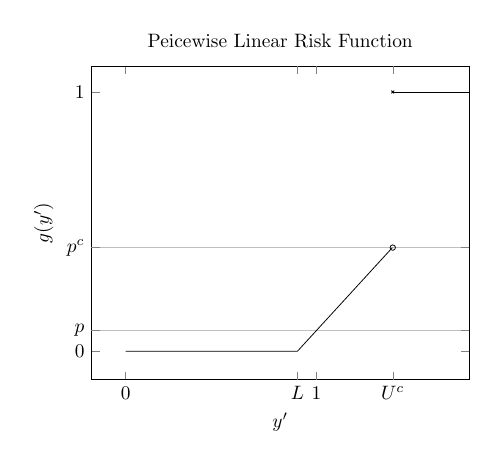
\begin{tikzpicture}[scale=.7]
      \begin{axis}[ 
	  xlabel=$y'$,
	  ylabel=$g(y')$,
	  title = Peicewise Linear Risk Function,
	  unbounded coords = jump,
	  xtick= {0},
	  ytick= {0, 1},
	  extra y ticks={.08,.4},
	  extra y tick style={grid=major},
	  extra y tick labels={$p$,$p^c$},
	  extra x ticks={.9,1,1.4},
	  extra x tick labels={$L$, 1, $U^c$},
          xmax=1.8,
          ymax=1.1,
          scatter/classes={
 	    a={mark=o,line width=3pt,scale=.75},%
 	    b={mark=o,line width=1pt,scale=1.25}%
	}]
	\addplot[black] coordinates { 
	  (0,0)		
	  (.9,0)	
	  (1.3975,.3995)		
	};	
        \addplot[black,mark=x,mark size=1pt] coordinates { (1.4,1) (2.5, 1)};
        \addplot[black,mark=o,mark size=1.4pt] coordinates{(1.4,.4)};
      \end{axis}
    \end{tikzpicture}


\subsubsection*{Line Risk Function}
The risk function $g : \R \rightarrow \R$ takes the normalized flow $\hy_e$ and returns the risk $z_e = g(y_e)$ of the line.  
\begin{equation}
 g(\hy_e) = \bP{\Xi}{\text{Line }e\text{ fails} | \hy_e} 
\end{equation}
A piecewise linear function captures some of the important features of the endogenous risk of the transmission element.  Up to a certain point, $L$, the power flow does not add any risk above that of its normal outage rate.  Above that point, the additional risk is proportional to the additonal flow on the line.  One a critical capacity $U^c$ is reached, a protective element will trip and the line will fail with certainty (ignoring hidden failures).  
\begin{equation}\label{pwl_risk}
g(\hy_e) = \left\{ \begin{array}{l l}
  0 & \hy_e \leq L \\
  a + b \hy_e & L \leq \hy_e < U^c \\
  1 & U^c \leq \hy_e 
\end{array}
\right.
\end{equation}
The risk parameters $(L, p)$ will be fixed among all lines and  $a$ and $b$ can be calculated given the risk parameters $L,p$. 
% ----------- Piecewise Linear Parameter Calculations -----------------
\endnote{\textbf{Piecewise Linear Function Parameters}

The x intercept snf slope for the line risk function can be calculated as follows.\[a = -\frac{pL}{1-L}\] \[b = \frac{p}{1-L}\]}
The extension to line specific values is straightforward given the data and could be grouped based off line voltages and material parameters.

\subsubsection*{System Risk Measure}
First, we will define a risk measures in a static setting which can be solved for exactly using nonlinear programming. This risk measure can be weighted to account for importance of lines, which is useful in a cascading failure setting.
% ---------- Cascade ENDNOTE --------------
\endnote{\textbf{No Cascade Risk Measure}

While it is important that no lines fail, it may be overly restrictive while not actually reducing the risk of large load shedding events, which is the main concern from a system reliability perspective. It would certainly be more beneficial to keep the large high voltage lines in operation that are critical to system stability versus a few small distribution feeders, which may cause some small load shedding but would keep the bad events contained.  In this case, we would like to find the probability of no cascade given an power system operating point.  We can condition this probability on the events of individual lines failing, which we have used previously.
\begin{equation*}
P(\mbox{cascade}|x) = \sum_e P(\mbox{cascade}|e\mbox{ fails}) P(e\mbox{ fails}|x)
\end{equation*}
where $x$ is the operating point and here we worry about the flows $y$ and not the risk from generators.  Let $q_e(y_e) = P(\mbox{cascade}|e\mbox{ fails})$, then we have
\begin{equation} 
H^c(y) = \prod_{e \in \cE} \left( 1 - g_e(y_e)q_e(y_e) \right) \geq 1 - \epsilon
  \end{equation}  
The conditional probabilities $q_e(y_e)$ act as weights on the probability of line failures, so if we set them all to 1 to put an equal importance on every line, we get back our previous formulation.
} 
% -----END------ Cascade ENDNOTE -------END-----
Then, the risk measure is extended to random variables $\rz_e = g( \hry_e )$.

Let $h(z) : \R_+^M \rightarrow \left[ 0, 1 \right]$ be the risk function dependent on individual line risk $z$ which is defined by
\[ h(z) = P_\Xi \left[ \mbox{no line fails} \right] \]
where the probability space $\Xi$ is orthogonal to that of demand ($\Omega$) and can be thought of as an effective capacity.  That is, the line will fail if it has flow above its effective capacity.  The space $\Xi$ will then represent transmission elements effective capacity distribution.  

This risk measure defines a bernoulli random variable that takes on the value 1 with probability $h(z)$.  By multiplying the probabilities that individual lines succeed $(1-z_e)$, we have the probability that all lines succeed
\begin{equation}  \label{nofail}
h(z) = \prod_{e \in \cE} \left( 1 - z_e \right)
\end{equation}  
where $z_e$ is the probability that line $e$ fails.  Also, we restrict $z_e \in [0,1)$ since when $z_e = 1$ for any line, we know that the probability no line fails is 0.  This implies that an individual line will have a hard line limit (denoted $U^\epsilon$) related to the system risk $\epsilon$.
% ---------------- Hard Line Limits ENDNOTE --------------------
\endnote{\textbf{Hard Line Limits}

There is a notion of maximum line limits in this model, however these line limits can not be attained simultaneously as is true with the current model.  Using the no failure risk measure \ref{nofail} and bounding according to some risk tolerance $\epsilon$, we have
\[ \prod_{e \in \cE} (1-z_e) \geq 1 - \epsilon \]
\[ \sum_{e \in \cE} \ln \left( 1-z_e \right) \geq \ln \left(1-\epsilon \right) \]
where the second constraint is an equivalent formulation using logarithms.
Then we note that all the terms are non-positive, so that the constraint must hold term by term, which gives
\[ \ln \left( 1 - g_e(y_e)  \right) \geq \ln \left( 1- \epsilon \right) \]
\begin{equation*}
g_e(y_e) \leq \epsilon
\end{equation*}
where the second inequality comes from taking exponentials of both sides and reducing. The line will have critical risk $\epsilon$ when $g_e(y_e) = \epsilon$, so that the hard line limits
\begin{equation} \label{hardline}
U^{\epsilon} = g^{-1}\left(\epsilon\right)
\end{equation}
will be an upper bound on line flow.
}
% ----END---------- Hard Line Limits ENDNOTE -----------END-----
This function can be solved exactly for static demand using nonlinear programming by taking a log transform of the line risk.
% ----------------- Exact Solution for Static Demand ENDNOTE ----------------
\endnote{\textbf{Static Demand, Exact Solution}

The system risk constraint can be written
\begin{equation*} H(y) = \prod_{e \in \cE} \left( 1 - g_e(y_e) \right) \geq 1 - \epsilon
  \end{equation*}  
where $1 - g_e(y_e)$ is the probability that line $e$ doesn't fail given flow $y_e$, and taking the product of all these events gives the probability that no lines fail.  We have
\begin{align*}
  \ln \left( \prod_{e \in \cE}\left( 1 - g_e(y_e)\right) \right) &\geq \ln \left(  1 - \epsilon \right)  & g_e(y_e) \in [0,1) \forall e  \\
  \sum_{e \in \cE} \ln \left( 1-g_e(y_e) \right)  &\geq \ln \left( 1- \epsilon \right) & g_e(y_e) \in [0,1) \forall e 
\end{align*}
Letting $w_e = \ln \left( 1 -g_e(y_e) \right)$ take the value of a transformed line risk, we get our risk constraint
\begin{equation} \label{cceqn}
\sum_{e \in \cE} w_e \geq \ln \left( 1-\epsilon \right)
\end{equation}
with
\begin{align*}
w_e &= \ln \left( 1 - g_e(y_e)\right) \\
e^{w_e} &= 1-g_e(y_e) \\
g_e(x_e) + e^{w_e} &= 1 
\end{align*}
where $e^{w_e}$ is exponential function versus the subscript denoting the line.

And if we wanted to relax the constraint on $w_e$, we have $w_e \leq \ln \left( 1 - q_e(y_e) \right)$ since $w_e$ is related to the probability of success and lowering it would make it worse (and the real number would always satisfy the original constraint).
\begin{equation*}
g_e(y_e) + e^{w_e} \leq 1
\end{equation*}

\begin{figure}
\begin{center} 
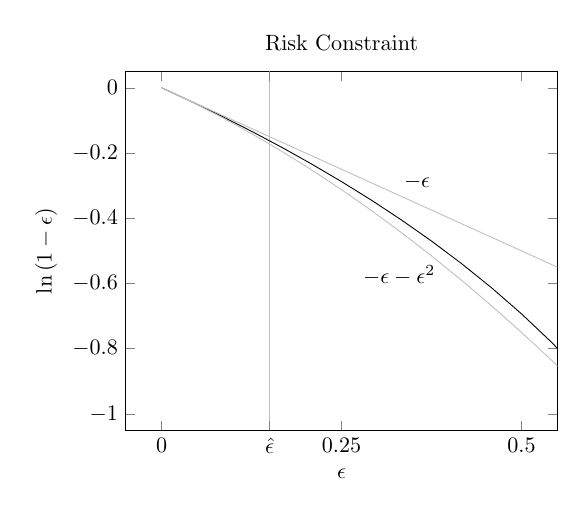
\begin{tikzpicture}[scale=.8]
\begin{axis}[ title=Risk Constraint,xlabel=$\epsilon$,ylabel=$\ln \left( 1-\epsilon \right)$,
  xmin=-.05,xmax=.55,
  ymin=-1.05,ymax=.05,
  xtick={0,.25,.5},
  	extra x ticks={.15},
	extra x tick style={grid=major},
	extra x tick labels={$\hat{\epsilon}$}
]
 \addplot[domain=0:.9999] { ln(1-x) };
 \addplot[domain=0:1,lightgray] {-x};
 \addplot[domain=0:1,lightgray] {-x - x^2};
  \node at (axis cs: .355,-.29) { $-\epsilon$};
  \node at (axis cs: .33,-.575) { $-\epsilon-\epsilon^2$};
\end{axis}
\end{tikzpicture}
\end{center}
\caption{Line risk substitution for individual branches}
\end{figure}
}
% --------END--------- Exact Solution for Static Demand ENDNOTE -------END---------
The function can be approximated by using a linearization of $h(z)$,
% -------------------- Linearization for Small Epsilon ENDNOTE -------------------
\endnote{\textbf{Linearization of Line Risk}

To find the linearization for small $t$, the taylor expansion $f(t)=f(t) + \grad f (a)(t-a) +...$ around $a=0$ will be useful.  Applying the taylor expansion to our risk measure \ref{nofail}, we end with the linear approximation
\begin{equation}\label{linear}
h(z) \approx 1 - \sum_e z_e
\end{equation}
%by using the partial derivative of $H(z)$    %%  + \frac{1}{2} (t-a)^T \grad^2 f(a)(t-a)  <---- Quadratic term
%\[ \frac{\partial}{\partial z_{e'}} H ( z ) = \prod_{e \neq e'} (1-z_e) ( -1 )\]
%and $\grad H(0) = -1$.
It is important to note that the linear approximation underestimates system risk and the quadratic approximation overestimates risk for small risk $h(z)$.

The risk can also be bounded using the Bonferroni Inequalities, which is a generalization of Boole's Inequality, or the union bound.
}
% -----END--------------- Linearization for Small Epsilon ENDNOTE ------------END-------
which recovers the model used by Wang et. al \cite{wang_2013}.

\subsubsection*{System Risk for Random Variables}
The system risk $r$, which is the probability that one or more lines fail, is the compliment of $h(z)$.  Applying the line risk function \ref{pwl_risk} to the system risk measure \ref{nofail} and integrating over the volatile injection space $\Omega$, we have
\begin{equation*}
1- r = \E{\Omega}{ \prod_{e \in \cE} (1 - g(\hry_e) )}
\end{equation*}
and applying the linear approximation \ref{linear} we get the total risk measure
\begin{equation}
r = 1 - h(z) \approx \sum_{e \in \cE} \E{\Omega}{g(\hry_e)}
\end{equation}
by exchanging summation and expectation of the approximated risk function. 

%\subsubsection*{Expectation of a Truncated Gaussian}
The system risk contributed by line $e$ is integrated over the space orthogonal to exogeneous events.  This will capture the risk from system decision, specifically how much power is flowing through that particular arc.  

\subsubsection*{Line Risk for Gaussian Flows}
Let $ z_e = \E{\Omega}{g(\ry_e)} $ be the individual line risk. We can break $z_e$ into three segments based upon the piecewise linear function \ref{pwl_risk}.  The first segment for $\hry_e \leq L$ takes the value zero, the second segment, for $L \leq \hry_e \leq U^c$, takes an expected value of a truncated normal distribution, and the last segment, $U^c \leq \hry_e$, takes one with a CDF evaluation of a normal distribution.  That is
\[ z_e = \E{\Omega}{ a+b\hry_e | L \leq \hry_e \leq U^c } \bP{\Omega}{L\leq \hry_e \leq U^c}  + \bP{\Omega}{ U^c \leq \hry_e } \] 

 The truncation from the critical capacity $U^c$, the level at which the line fails with certainty, can be ignored since we will stay far away from that point anyway.  This will be a reasonable assumption when $ (U^c - U^{\epsilon} )/\sigma $ is large, where $U^\epsilon$ is the level at which line risk is equal to the system risk tolerance.  Then, we have
\[ z_e = \E{\Omega}{ a+b\hry_e | L \leq \hry_e } \bP{\Omega}{L\leq \hry_e} \]

The branch flows are truncated gaussian, which have known mean and variances.
\endnote{\textbf{Truncated Gaussians}

Truncated gaussian's mean and covariance are known to be
\[  \E{\Omega}{ \hry_e | L \leq \hry_e } = \mu^y_e + \frac{\phi( \alpha_L )}{ 1- \Phi(\alpha_L)} \sigma^y_e \]
\[ \bP{\Omega}{ L \leq \hry_e } = 1 - \Phi(\alpha_L) \]
where $\alpha_L = \frac{L - \mu^y_e}{\sigma^y_e}$, the PDF $\phi(\cdot)$ , and the CDF $\Phi(\cdot)$ are for the standard normal distribution.  
}
The line risk is a function of the mean and covariance of the branch flows.  The line risk expression is then
\begin{equation}\label{line_risk}
z_e(\mu^y_e,\sigma^y_e) = (a + b \mu^y_e)\left[ 1 - \Phi(\alpha_L) \right]  + b \sigma^y_e \phi(\alpha_L) 
\end{equation}
which is a convex function with respect to $\mu^y_e$ and $\sigma^y_e$. 
% -------------- Convex Line Risk ENDNOTE ---------------------
\endnote{\textbf{Convex Line Risk}

The line risk is
\begin{equation}
z_e(\mu^y_e,\sigma^y_e) = (a + b \mu^y_e)\left[ 1 - \Phi(\alpha_L) \right]  + b \sigma^y_e \phi(\alpha_L) 
\end{equation}
Taking the derivatives of $z$ with respect to $\mu^y_e$ and $\sigma^y_e$, we have
\begin{align*}
\frac{\partial z_e}{\partial \mu}(\mu^y_e,\sigma^y_e) & = b\left[ 1 - \Phi(\alpha_L) \right]\\
\frac{\partial z_e}{\partial \sigma}(\mu^y_e,\sigma^y_e) & = b \phi(\alpha_L) 
\end{align*} 
The Hessian is found with the second derivatives and is given by
\begin{equation}
\cH_z(\mu^y_e,\sigma^y_e) = \frac{b \phi(\alpha_L)}{\sigma}
\left[ 
\begin{array}{c c}
1 & \alpha_L \\
\alpha_L & \alpha_L^2
\end{array}
\right]
\end{equation}
Then, we note that the determinant is 0 and the diagonal elements are positive so that there is a positive eigenvalue and a zero eigenvalue, thus the line risk is convex with respect to $\mu^y_e, \sigma^y_e$.  Since system risk is approximated by the sum of line risks, this system risk measure is convex.
}
% ---END----------- Convex Line Risk ENDNOTE -----------------END----

%%%%%%%% Section 3
\section{Dispatch Models for Bulk Power Systems}
Bulk power systems rely on dispatch models to clear the markets for power in a timely manner.  These models are critical to ensure that market is cleared minimizing cost while maintaining a set of reliability constraints.  In its most common for, the DC power flow model is used to clear economic markets for both real-time and day-ahead operation, where the day-ahead operation has the additional complexity of committing slow ramping resources.  The set of reliability constraints traditionally refer to line thresholds that the system must maintain continuously as well as the systems resiliency to N-1 contingencies.  First, a brief overview of the three models will be given and then the full mathematical programming models for each will be given.  A mention of their extension to exogenous contingencies will be given and then the solution methodology will follow.

\subsection{Overview of Models}
A primary difference between the Optimal Power Flow model and the Joint Chance Constraint model is that the OPF model constrains line risk and the JCC model constrains system risk.  The OPF model is typically done in a static sense where as the JCC model involves uncertainty. The CC model is the extension of OPF under uncertainty.
\begin{description}
\item[Optimal Power Flow (OPF)] This model is used to clear real-time markets for bulk power systems.  It has fixed thresholds for line capacities.  All power flows are assumed to be static.  The regular DC power flow assumptions are used.  The objective is to minimize cost for feasible injects that do not violate line capacity thresholds.
\item[Chance Constraint (CC)] This model assumes a covariance matrix for volatile injects and places probabilistic constraints on line capacity thresholds.  For an arbitrary slack distribution, the standard deviation for line flows can be represent as a second order cone with respect to the slack distribution variables.
\item[Joint Chance Constraint (JCC)] This model replaces line capacity thresholds with line risk measures.  The system risk is the sum of individual line risks.  The objective is to minimize cost for feasible injects that do not violate a system risk threshold.
\end{description}

\subsubsection*{OPF Model}
The OPF model uses the DC simplifications from the full AC model to ensure the model can be solved reliably in a timely manner.  A standard OPF model will be shown here and used for the computational section.
\begin{subequations}
\label{opf_program}
\begin{alignat}{3}
\min_{\left(x,\beta,;\theta,y\right)} && \multispan{2}{$\displaystyle\sum_j \left[  c_2 \left(x_j^2 + \beta_j^2 \sD \right) + c_1 x_j + c_0 \right]$}  & \label{jcc_obj}\\
                        && \textstyle \sum_j c^g_{ij} x_j - \sum_j c^b_{ie} y_e          &=d_i       && \forall i \label{opf_cons}\\ 
                 && y_e - b_e \textstyle \sum_i c^b_{ie} \theta_i          &=0         && \forall e \label{opf_kcl}\\
                 && y_e &\in \left[ -U_e, U_e \right] && \forall e \label{opf_limit}\\
                 && x_j &\in \left[ G^{min}_j, G^{max}_j \right] && \forall j  \label{opf_gen}  
\end{alignat}
\end{subequations}

\subsubsection*{CC Model}
The CC model extends OPF to the case with uncertainty in net injects.  The line constraints \ref{opf_limit} will be replaced by probabilistic constraints and additional constraints will be added to describe the slack distribution, standard deviations of branch flows, and probabilistic generator constraint.
\begin{subequations}
\label{opf_program}
\begin{alignat}{3}
                 && y_e + s_e \eta_l &\in \left[ U_e, U_e \right] && \forall j  \label{cc_line}   \\
                 && \pe - \textstyle \sum_j A_{ej} \beta_j   &=0 &&\forall e \label{cc_pi}\\ 
                 && s^2_e - \pi_e^2 \sD + 2 \pi_e \se      &\geq\see &&\forall e \label{cc_var} \\
                 && x_j + \beta_j \sigma_\Delta \eta_g &\in \left[ G^{min}_j, G^{max}_j \right] && \forall j  \label{cc_gen}   \\
                 && \textstyle \sum_j \beta_j &=1 && \label{cc_slack}
\end{alignat}
\end{subequations}
\subsection{Joint Chance Constraint Model}%WITH ARBITRARY SLACK!!
The JCC model departs from traditional power flow models in that it allows for a trade-off between line risk and system risk. Since the cost and risk are both related to the slack distribution, the model will be given with the slack distribution as a variable.  In this section, the full joint chance constraint model will be given followed by a brief explanation of some of the constraints.  The relevant parameters derived from the injection covariance matrix will also be given.  Then a cutting plane algorithm will be shown to solve the full JCC model.

\begin{subequations}
\label{jcc_program}
\begin{alignat}{3}
\min_{\left(x,\beta,;\theta,y,\pi,s,z\right)} && \multispan{2}{$\displaystyle\sum_j \left[  c_2 \left(x_j^2 + \beta_j^2 \sD \right) + c_1 x_j + c_0 \right]$}  & \label{jcc_obj}\\
                        && \textstyle \sum_j c^g_{ij} x_j - \sum_j c^b_{ie} y_e          &=d_i       && \forall i \label{jcc_cons}\\ 
                 && y_e - b_e \textstyle \sum_i c^b_{ie} \theta_i          &=0         && \forall e \label{jcc_kcl}\\
                 && y_e &\in \left[ -U_e^\epsilon, U^\epsilon_e \right] && \forall e \label{jcc_limit}\\
                 && x_j + \beta_j \sD \eta_g &\in \left[ G^{min}_j, G^{max}_j \right] && \forall j  \label{jcc_gen}   \\
                 && \textstyle \sum_j \beta_j &=1 && \label{jcc_slack}\\
                 && \pe - \textstyle \sum_j A_{ej} \beta_j   &=0 &&\forall e \label{jcc_pi}\\ 
                 && s^2_e - \pi_e^2 \sD + 2 \pi_e \se      &\geq\see &&\forall e \label{jcc_var}\\
                 && z_e - g(|y_e|,s_e)  &\geq 0 && \forall e \label{jcc_lr}\\
                 && \textstyle \sum_e z_e &\leq \epsilon && \label{jcc_risk}
\end{alignat}
\end{subequations}

The objective \ref{jcc_obj} for the JCC model is the typical quadratic objective for the OPF model plus a contribution from the slack distribution due to the uncertainty in the volatile injects.  This objective is the expected cost of meeting the realized demand.  The uncertainty in demand also causes the generator constraint \ref{jcc_gen} to be probabilistic with $\eta_g = \Phi^{-1}(1-\epsilon_g)$ being its tolerance.  The upper and lower bounds $[G^{min},G^{max}]$ will be dependent on many things, most importantly the time frame used.  This will be affected by the status of the generator (on,off,starting up,shutting down) and its ramping rate as well as any physical limits it may have.  

The first equations \cref{jcc_obj,jcc_cons,jcc_kcl,jcc_slack,jcc_limit,jcc_gen} are your typical DC power flow and the last set \cref{jcc_pi,jcc_var,jcc_lr,jcc_risk} describe system risk.  The branch variance equations \ref{jcc_var} are a second order cone and the line risk equations \ref{jcc_lr} involve the CDF of a normal distribution.  These equations will be solved via a cutting plane approach so that the individual subproblems will be linear programs.


\subsubsection*{Branch Response Parameters}
The volatile injects have mean 0 and a covariance matrix $\Sigma^m$.  This covariance matrix is used to describe parameters for relating the injection covariance matrix to the branch covariance matrix needed for line risk.  The variance in lines is due to a combination of the volatile injects and the slack distributions response.  The following parameters are used in JCC \ref{jcc_program} and the cutting planes \ref{branch_var_cuts}.
\begin{subequations}
\begin{align}
 \sD &= \sko \skt \sigot  \\
 \se &= \sko \skt A_{ek_1} \sigot \\
 \sen &= \sko \skt A_{ek_1} A_{nk_2} \sigot
\end{align}
\end{subequations}


\subsection{Exogenous Contingencies}
The JCC model also has a straightforward extension to exogenous contingencies.  In the computational experiments, each model will have a respective N-1 version which ensures the system is stable after any single line goes out.  In order to explore this model, line outage factors are used, which are linear shift factors for branch flows.  Using these, constraints will be formed on the second stage branch flow variables.  The mean branch flow as well as standard deviation of flow can be calculated.  In the OPF version, hard line constraints are used.  In the CC version, probabilistic constraints are formed for line flow.  Finally, the JCC version enforces a system risk constraint on each N-1 subsystem.  In all versions, the respective constraints are loosened in the second stage.

The implementation as well as solution method, which closely parallel the base case, are given in the appendix.
% --------------- Exogeneous Contingency Details ENDNOTE ----------------
\endnote{\textbf{Exogenous Contingency Details}


The mean branch flows for line $e$ given contingeny $n$ can be found by
\begin{equation}
 \ry_e^n = \ry_e + L_{e n} \ry_n 
\end{equation}
with $L_{en}$ being a line outage factor for outage $n$'s effect on line $e$.


}
% -----END---------- Exogeneous Contingency Details ENDNOTE -------END---------


\subsection{Solution Method}
Due to the inclusion of non-analytic functions (the line risk function), an out of the box solver would not work.  However, the risk function is convex, so cutting planes were chosen for the solution methodology.  In addition, there were many second order cone constraints (number of lines).  Instead of using these constraints explicitly, they were added indirectly through cutting planes as well.  This kept the program to a manageable size and allowed for fast solve times.  When exogenous contingencies are added, cutting planes are extremely efficient since no constraints will be added for lines without risk.


\subsubsection*{Risk Function for Transmission Lines}
The line risk constraint \ref{jcc_lr} involving the CDF function for a normal distribution rules out many potential solving options.  Since the equations are convex, we can solve this using a cutting plane approach to describe the line risk in terms of the mean branch flow $y_e$ and the standard deviation of branch flow $s_e$.  While there are infinitely many cuts, this program can be solved for a given error tolerance with a finite, and typically small, set of cuts.
\begin{subequations}
\label{line_risk_cuts}
\begin{align}
z_e \geq g(\hye,\hse) &+ \frac{\partial g}{\partial y_e}(\hye,\hse) \left(y_e - \hye \right) 
+ \frac{\partial g}{\partial s_e}(\hye,\hse) \left(s_e - \hse \right) \\
g(y_e,s_e) &= (a + b y_e)\left[ 1 - \Phi(\alpha_L) \right]  + b s_e \phi(\alpha_L)  \\
 \frac{\partial}{\partial y_e}g(y_e,s_e) &= b\left[ 1 - \Phi(\alpha_L) \right]\\
\frac{\partial}{\partial s_e}g(y_e,s_e) &= b \phi(\alpha_L) 
\end{align}
\end{subequations}


\subsubsection*{Branch Variance Constraints}
The standard deviation of branch flow can be formulated as a second order cone with respect to the slack distribution variables.  While this could be solved with an out of the box solver, we proceed with a cutting plane approach to speed up solve times.  As the solution approach is already iteratively improving system risk, it adds only a small amount of work to add these cuts as well.
\begin{subequations}
\label{branch_var_cuts}
\begin{align}
s_e \geq \fehb &+ \sum_j \pfehb \left( \beta_j - \hat{\beta_j} \right)\\
  \feb &= \sqrt{\pe^2 \sD - 2 \pe \se  + \see }\\
  \pfeb &= \frac{A_{ej} \left( \pe \sD - \se \right)}{\sqrt{\pe^2 \sD - 2 \pe \se  + \see }}
\end{align}
\end{subequations}

\subsubsection*{Cutting Plane Algorithm}
Now, we can describe the cutting plane algorithm for JCC at a high level and give pseudo-code \ref{jcc_alg} for implementation.  The main subproblem the algorithm will solve is the standard DC power flow.  After solving, the generator injects $x$, slack distribution $\beta$, and branch flows $y$ will be used to calculate risk information about the dispatch point.  To get the risk information, the branch standard deviations $s$ need to be calculated.  With the mean flow $y$ and standard deviation $s$, the line risk $z$ can be calculated.  The sum of line risk is system risk $r$.  If $r$ is less than the required system risk $\epsilon$, the problem is solved.  Otherwise, the algorithm will add cuts for all lines with a positive risk $z$.  The cuts will describe how $z$ is related to $y,s$ and how $s$ is related to $\beta$.  Then the power flow subproblem will be solved with the addition of the cuts and this will repeat until it is infeasible or the risk constraint is satisfied.
\begin{algorithm}
\caption{This cutting plane algorithm solves JCC \ref{jcc_program} via linear programs and cutting planes}\label{jcc_alg}
\begin{algorithmic}
\Procedure{JCC}{d,$\Sigma^m$,$\epsilon$,$\epsilon_g$,L,p}
\State $L \gets \emptyset$  (Set of Lines with potential risk)
\State $S \gets \emptyset$  (Set of Cuts)
\State $r \gets 0$ (Risk)
\BState \emph{solve}:
\State $(\hat{x},\hat{\beta},\hat{y}) \gets $Solve DC Power Flow, \cref{jcc_obj,jcc_cons,jcc_kcl,jcc_slack,jcc_limit,jcc_gen}, with cuts $S$, risk $r\leq\epsilon$
\If {Infeasible} \Return Problem Infeasible 
\EndIf
\State Calculate $\hat{s},\hat{z},\hat{r}$ using $(\hat{x},\hat{\beta},\hat{y})$ and \cref{branch_cov,line_risk}
\If {$\hat{r} \leq \epsilon + tol$} \Return Optimal $(\hat{x},\hat{\beta},\hat{y},\hat{s},\hat{z},\hat{r})$
\EndIf
\For{$\forall e$}
\If {$\hat{z_e} \geq tol$}
    \If {$e \notin L$}
            \State $L \gets \left\{L,e\right\}$
            \State Initialize $s_e,z_e$
            \State $r \gets r + z_e$
    \EndIf            
    \State $S \gets$ line risk cuts \ref{line_risk_cuts} for $z_e,y_e,s_e$ dependent on $\hat{z}_e,\hat{y}_e,\hat{s}_e$
    \State $S \gets$ branch variance cuts \ref{branch_var_cuts} for $s_e,\beta_e$ dependent on $\hat{s}_e,\hat{\beta}_e$
\EndIf
\EndFor
\State \textbf{goto} \emph{solve}
\EndProcedure
\end{algorithmic}
\end{algorithm}





%%%%%%%% Section 5
\section{Computational Experiments}
This section will explain the computation setup, the test cases, the experiments performed, and the intuition to gain from the comparison of OPF, CC, and JCC models.
\subsection{Implementation of the JCC Model}
All of the experiments are run on a laptop with an Intel i7-3537U processor with 2 cores,4 threads at 2.00GHz.  The laptop has 8GiB of memory, but even with the large case files (2383 nodes), memory is not an issue.  The laptop is running Linux Mint Petra 16.  The OPF, CC, and JCC models are all solved within a C++ program.  The program uses Armadillo\cite{armadillo} for linear algebra and Concert and CPLEX to solve the linear programs.  CPLEX is run with default settings and the dual simplex algorithm is used to solve the linear programs (quadratic objective for the small case).  All time comparisons are using the same system environment with a fixed clocked speed and few programs in background.  The primary DC OPF solver in the C++ program has been developed to output nearly identical results to Matpower.\cite{matpower} 
\subsection{Single Instance}
The test cases are all pulled from Matpower test cases.  The two test cases used will be the 30 bus test case as well as the 2383wp test case.  The small test case will be used to show some properties of the different dispatch points and the cost-risk frontier.  The large test case will be used for time trials as well as a cost-risk scatter plot.  

\subsubsection*{30 Bus Case}
This case from Matpower has 30 buses, 41 branches, and 6 generators.  The branches have a single capacity rating and in the given demand scenario does not have active line constraints.  A capacity factor $M$ will be used to uniformly scale the branch capacities.  All of the generators are active and have quadratic cost functions.  Ramping constraints for generators are not considered and the generators are allowed to take any value in its given range (the probabilistic generator constraints are ignored to focus on branch constraints).  In addition, all generators will be allowed to participate in the slack distribution.  Each bus with a demand will be considered volatile, with mean equal to the demand.  For this example, the injections will be independent of each other but this need not be the case.  The variance of each injection is equal to 5\% of the demand at the node times a budget factor $B$.

\begin{table}
\centering
\begin{tabular}{ |c| c c c |}
\hline
& OPF & CC & JCC \\
\hline
\hline
Cost & 567.1 & 574.0 & 565.2\\
$r$ & 0.0171 & 0.0179 & 0.0080\\
\hline
\end{tabular}
\caption{Cost and risk results for OPF,CC, and JCC models on the small test case}\label{solve_results}
\end{table}

\begin{table}
\centering
\begin{tabular}{| c| c |c c c c c c |}
\hline
 & Mod & g1 & g2 & g3 & g4 & g5 & g6 \\
\hline
\hline
$\left[ g_{min}, g_{max} \right]$& & [0,80]&[0,80] &[0,50] &[0,55] &[0,30] &[0,40]  \\
$\left\{ c_2, c_1 \right\}$ && $\left\{0.02,2\right\}$  &$\left\{0.0175,1.75\right\}$ &$\left\{0.0625,1\right\}$ &$\left\{0.00834,3.25\right\}$ &$\left\{0.025,3\right\}$ &$\left\{0.025,3\right\}$  \\
\hline
\hline
$x_g$ &OPF& 39.7  &  52.3  &  24.2  &  35.7  &  19  &  18.3   \\
$x_g$ &CC& 35.9  &  47.9  &  25.7  &  37.2  &  19.3  &  23.1    \\
$x_g$ &JCC& 41.9  &  55.0  &  23.2  &  34.0  &  18.6  &  16.5    \\
\hline
$\beta_g$ &OPF& 0.1548  &  0.1769  &  0.0495  &  0.3712  &  0.1238  &  0.1238    \\
$\beta_g$ &CC& 0  &  0  &  0.4411  &  0.2986  &  0  &  0.2602   \\
$\beta_g$ &JCC& 0.2456  &  0.2795  &  0.0846  &  0.0646  &  0.0597  &  0.2659   \\
\hline
\end{tabular}
\caption{Generator results using OPF, CC, and JCC models on the small test case.}\label{solve_one}
\end{table}

The first example will have risk parameters $L=0.9$, that is a line will begin taking on risk after it is at 90\% of its rated capacity.  The factor $p=0.005$ means that at nominal capacity, the line will have a $0.5\%$ chance of failing.  The line capacities will be scaled by $M=0.745$. The system risk constraint will be $\epsilon=0.008$, that is a $0.8\%$ chance of one or more lines failing.  The chance constraint version of OPF will be defined by $\eta_L=0.05$, that is the line capacities can not be violated more than $5\%$ of the time.  Finally, the covariance matrix will be scaled by $B=0.025$ so that the stanadard deviation of aggregate demand is $0.6$, a small fraction of total demand $189.2$.  The results for $(x,b)$ are tabulated in \cref{solve_results,solve_one}.



The CC model is always more conservative then the OPF model as it will tighten the line constraints.  This means that the CC version will always be at least as expensive as the OPF model.  In this case, the total cost rose by \$7 to ensure the line constraints were met probabilistically (95\% of the time).  The JCC model was able to lower the cost because it removed the branch capacity constraints (or increased them by 6\% to match the system risk level).  In addition, JCC knows and constrains the system risk measure so that it is able to find a cheaper point with a system risk level half that of the OPF and CC models.



Another interesting feature is that the slack would like to be distributed as much as possible to reduce cost.  This can be seen from the objective \ref{jcc_obj} due to the squared beta term and the OPF results show it spreading when there is no concerns of line or system risk.  The CC model slightly changes it's generator position as well as removing 3 generators from the slack distribution.  It is removing generators which have an effect on the probabilistically constrained transmission lines in order to ensure that the constraints are met $95\%$ of the time.  The JCC model has moved in almost exactly the opposite direction and has kept a distributed slack.




\subsubsection*{Cost-Risk Frontier}
  \begin{figure} % redo with new operating models
\centering
\begin{tikzpicture}
\begin{axis}[title=Cost vs Risk (case30),scale=1, xlabel=Cost, ylabel=Risk, legend pos=outer north east]
\addplot+[opacity=.7,mark size=1] table[x=copf,y=ropf] {data/cost-risk2.dat};
\addlegendentry{OPF}
\addplot+[opacity=.7, mark size=.1] table[x=ccc,y=rcc] {data/cost-risk2.dat};
\addlegendentry{CC}
\addplot+[opacity=.7, mark size=.1] table[x=csjc,y=rsjc] {data/cost-risk2.dat};
\addlegendentry{JCC}
\end{axis}
\end{tikzpicture}
\caption{Reliability frontier for the small test case}\label{costriskfront}
\end{figure}
%pow case/30.db  .775 1.1 1 .00195 .4 .00275 .5 .9 .005 .4 1000 2> cost-risk.dat
%m0   m1          mg   eps epsN     pL pG     L  p  B    T
%0.775            1.1  1   0.00195  0.4       0.00275    0.5     0.9     0.005   0.4     1000
Now we will use this same example case to draw a cost-risk frontier.  An efficient operating point would be at that boundary of the feasible points, that is, neither cost nor risk can be improved without a loss to the other.  Since neither the OPF or CC model uses or constrains our risk measure, it would be unlikely for them to be on the boundary.  In figure \ref{costriskfront} we see that this is the case.  The OPF model is in the interior and is equivalent to the CC model when $\eta_l=.5$.  Since the branch flows are gaussian, if the mean flow is at its threshold, it has a 50\% chance of being over its threshold.  As $\eta_l$ is reduced, the CC line is drawn.  The JCC line is started by finding the point when the system risk level is not constrained, for this case $r=.01$.  As $r$ is decreased, the system risk becomes constrained and the cost begins to rise as the risk level is reduced.


It is important to note that the cost-risk frontier is entirely dependent on how system risk is measured.  In our case, we use a piecewise linear failure density function with parameters $L$ and $p$.  As $L$ and $p$ are varied, the shape of these frontiers will change.  Holding $p$ fixed and increases $L$ towards 1, the CC model, while still on the interior of the frontier, does a better job of reducing system risk.  With $L$ around .98 (this will depend on the variance of aggregated injects), the CC and the JCC behave similar.  Both programs will try to reduce the flow of lines that are at their capacity, with the exception that JCC will allow a small number, typically one, of these lines to increase.  More discussion on this behavior will be given in the sensitivity analysis section \ref{senseanal}


\subsubsection*{2383wp Bus Case}
This case from Matpower has 2383 buses, 2896 branches, and 327 generators.  The case is similar to the small case in many respects, such as only a single line rating capacity being given.  The generators have the biggest difference in that there are many which are nearly fixed and have no cost.  The larger flexible generators are only given a linear cost so that there is no quadratic objective.  The covariance matrix will be developed the same as in the small case.

Running this case with parameters $M=1.03, \epsilon=0.03, \eta_L=0.05, L=0.85, p=0.005$, and $B=1$ and recording the standard cost and risk information as well as solve time.  The case was repeated 10 times and the mean time is reported in \ref{solve_time}.  CC and JCC take a similar amount of time, the majority of the work at each step being the calculation of the branch covariance matrix.  The total time will largely depend on how many iterations the algorithms take, which is typically around 5-7. 

In addition, we solved 100 instances with random demand and the same covariance matrix to show the speed-up you can achieve with repeated solves.  By having the same covariance matrix, all of the cuts for previous solves are still valid.  So, in addition to using a warm start on the LP, after the first few solves the algorithm typically needs no additional cuts.

\begin{table}
\centering
\begin{tabular}{| c| c c c| }
\hline
Time ($\eta_L,\epsilon$) & OPF & CC & JCC \\
\hline
\hline
Time (0.05,0.03)& 0.37  & 8.7 & 7.5 \\
%Time (0.10,0.05)& 0.37 & 8.6  & 7.4  \\
Time (0.20,0.07)& 0.37  & 8.4 & 8.0 \\
%Time (0.30,0.10)& 0.37  & 8.4 & 7.6 \\
Time (0.40,0.20)& 0.37  & 8.3 & 6.1 \\
%Time (0.45,0.30)& 0.37  & 8.3 & 6.1 \\
Time (0.48,0.30)& 0.37  & 7.7 & 6.1 \\
\hline
\hline
Avg Time (100 trials)& 0.34  & 2.2 & 2.3 \\
\hline
\end{tabular}
\caption{Time comparison, in seconds, for OPF,CC, and JCC on the large test instances.}\label{solve_time}
\end{table}

\subsubsection*{Line Threshold Comparison}
Here we will explore what the JCC model is doing to lower its cost or risk compared to the traditional models.  For this experiment, the parameters are as follows, $M=1.03, \epsilon=0.015, \eta_L=0.05, L=0.95, p=0.005$, and $B=1$.  Solving this program, we see that the majority of the lines are less than 50\% utilized.  There is a small number of lines that are at or near their nominal capacity.


\begin{tabular}{c c}
%\begin{figure}
%\centering
\begin{tikzpicture}[scale=.8]%1.3,1
\begin{axis}[title=Normalized Line Flow , xlabel=Line, ylabel=Line Flow (MW),xmin=0,xmax=9, grid=major,legend style={at={(.98,.875)},anchor=north east}]

                        \addplot+[opacity=.9,only marks, mark size=1, mark=triangle,
                        /pgfplots/error bars/.cd,
                        x dir=none,
                        y dir=both,
                        y explicit] table[x=count,y=opf, y error=eopf] {data/highflow.dat};
                        \addlegendentry{OPF}

                         \addplot+[opacity=.9,only marks, mark size=1, mark=o,
                        /pgfplots/error bars/.cd,
                        x dir=none,
                        y dir=both,
                        y explicit] table[x=count,y=cc, y error=ecc] {data/highflow.dat};
                        \addlegendentry{CC}

                        \addplot+[opacity=.9,only marks, mark size=1, mark=square,
                        /pgfplots/error bars/.cd,
                        x dir=none,
                        y dir=both,
                        y explicit] table[x=count,y=sjc, y error=esjc] {data/highflow.dat};
                        \addlegendentry{SJC}

\end{axis}
\begin{axis}[hide x axis, axis y line=right,ymin=-50,ymax=950,xmin=0,xmax=9,ylabel=Shadow Price (\$)]
   \addplot+[only marks,mark size=4,mark=star] table[x=count,y=dual] {data/duals.dat};
   \addlegendentry{Shadow Price (OPF)}
\end{axis}
\end{tikzpicture}
%\caption{All lines that have mean flow (in OPF) above 95\% of nominal capacity}\label{solve_shadow}
%\end{figure}
&
%\begin{figure}
%\centering
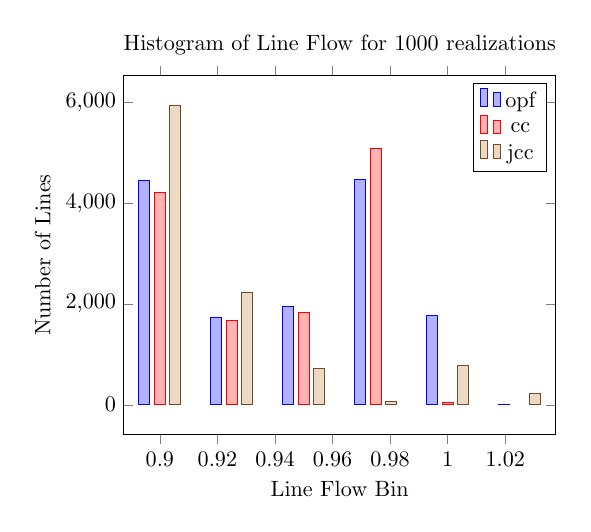
\begin{tikzpicture}[scale=.8]
\begin{axis}[title=Histogram of Line Flow for 1000 realizations, 
    xlabel=Line Flow Bin, 
    ylabel=Number of Lines,
x tick label style={
/pgf/number format/1000 sep=},
  ybar, bar width=5pt ,
  enlargelimits=0.1]
\addplot coordinates { ( 0.9,4450)  ( 0.925,1729)  ( 0.95,1949)  ( 0.975,4471)  ( 1,1770)  ( 1.025,3) };
\addplot coordinates { ( 0.9,4219)  ( 0.925,1678)  ( 0.95,1834)  ( 0.975,5077)  ( 1,53) };
\addplot coordinates { ( 0.9,5931)  ( 0.925,2218)  ( 0.95,711)  ( 0.975,70)  ( 1,784)  ( 1.025,221) };
\legend{opf,cc,jcc}
\end{axis}
\end{tikzpicture}
%\caption{Histogram to compare high flow lines of OPF,CC, and JCC}\label{histogram}
%\end{figure}
\end{tabular}

Now, we will look at the trade off that the JCC model is able to make due to it increasing the nominal line limit by 10\% to match the given system risk level.  In figure \ref{solve_shadow}, 8 lines are shown, which are lines above 95\% of their nominal capacity in the OPF model.  The mean line flows are plotted as well as the standard deviation based on the slack distribution for the solution.  
%There are 8 lines above 95\% of their capacity in the OPF model, indexed as lines 23,291,320,1380,1381,1815,2108, and 2109. 
In addition, the shadow prices for the original OPF model are shown for lines that are constrained.  In the OPF model, there are 3 lines at the nominal capacity.  Line 23 (index 1 in figure) has a dual price of 872, line 291 (index 2) has a dual price of 32, and line 2108 (index 8) has a dual price of 294.


In the CC model, these constraints are tightened further to ensure that these thresholds are met at least 95\% of the time.  The JCC model on the other hand relaxes these constraints and imposes a system risk constraint instead.  The final solution for the JCC model will have line 23 exceed its threshold with certainty but is rewarded with the high shadow price.  On the other hand, other lines with positive line risk may be restricted to ensure the system risk levels are met.

To give another perspective, the line flows were sampled and binned to create a histogram of line flows to show the trade-off between models.  For the JCC model, the line risk parameter $L$ was chosen to be 0.9.  The results can bee seen in figure \ref{histogram} where the bin size is $0.025$, for example the point $1$ is in reference to bin $1$ to $1.025$.  We can see that the normalized line flows pile up in bin 0.975 for the CC model and there are a number of lines in OPF that are in bin $1-1.025$, thus exceeding their capacity a significant amount of the time.  The JCC also has a line that exceeds its capacity, almost with certainty.  However, the JCC has far fewer lines that are at or near their capacity.



\subsection{Sensitivity Analysis}\label{senseanal}
Now, we want to look at the sensitivity of the JCC models to its input parameters and demand uncertainty.  First we will look at how the risk of the different dispatch points from the OPF, CC, and JCC models respond to changes in the failure density function parameters $L$ and $p$.  To this end, we solved the OPF, CC ($\eta_L=.01$), and JCC ($\epsilon=0.0003$, $L=.98$).  These three dispatch points are used to find the risk of the branch flows for varying risk parameters $L,p$. The cost of the dispatch points are tabulated in \ref{tabsense} and the sensitivity analysis is shown in figure \ref{figsense}. This figure shows that for the given JCC solution, the system risk stays under that of the CC model.  The OPF model has a lower cost so it is reasonable that the risk is much higher.  The same results were seen when polynomial risk functions were evaluated, such as $x^2,x^3,$ and $x^4$.


\begin{table}
\centering
 \begin{tabular}{ |c| c c c |}
\hline
& OPF & CC & JCC \\
\hline
\hline
Cost & 567.1 & 574.0 & 572.2\\
\hline
\end{tabular}
\caption{Table of cost for the three dispatch points used in the sensitivity analysis}\label{tabsense}
\end{table}


\begin{figure}
\centering
\begin{tikzpicture}[scale=.8]
\begin{axis}[title=L vs Risk, xlabel=L, ylabel=r,legend pos=outer north east,ymax=.04,xmin=.9,xmax=1,
	  extra x ticks={.98},
	  extra x tick style={grid=major},
	  extra x tick labels={}]


  \addplot+[opacity=.65,only marks, mark size=.35] table[x=L,y=ropf] {data/risk.dat};
  \addlegendentryexpanded{OPF}

  \addplot+[opacity=.65,only marks, mark size=.35] table[x=L,y=rcc] {data/risk.dat};
  \addlegendentryexpanded{CC}

  \addplot+[opacity=.65,only marks, mark size=.35] table[x=L,y=rsjc] {data/risk.dat};
  \addlegendentryexpanded{JCC}

\end{axis}
\end{tikzpicture}
\caption{A comparison of the three dispatch points for varying risk function parameters}\label{figsense}
\end{figure}






%%%%%%%% Section 6
\section{Conclusion and Future Work}

\subsection{Conclusion}
The primary strength of this model is the addition of a system risk constraint and the removal of line thresholds. Line thresholds are hard constraints that subject the system to price spikes.  The hard line constraints are somewhat arbitrary as the line will not fail when it is exceeded by a small amount.  Instead, an economic trade off should be made between individual lines to ensure the system risk is constrained at an adequate level.  The system risk measure allows for direct comparison of different dispatch points with respect to risk.

The JCC model is computationally efficient in its full form.  It allows for creation of a cost-risk frontier that finds dispatch points that are better in both terms of risk and cost.  Under uncertainty, this model should be compared against the CC model, which is a probabilistic interpretation of line thresholds.  Probabilistic line thresholds exacerbate the economic problems of hard constraints by further tightening the constraints.  In both of these models, the variable slack distribution plays a small direct role in cost through the objective, however is crucial in ensuring the line and system risk constraints are met.  
  
Combining the system risk measure and random power injects for the joint chance constrained model accounts for many things the traditional OPF model misses.  This model will give prices for system response to aggregated volatile injects, which is regulation and reserve support for different time periods.  Instead of having an ancillary service model which separates this, the JCC model directly accounts for it.  This will allow for valuing volatile injects, which will be important going forward as the grid integrates more uncertain generation (wind turbines) and demand (electric vehicles).

\subsection{Future Work}
There are many avenues to improve and extend this model.  One first question would be, what does the failure density function look like.  We used a piecewise linear model, but perhaps other models better represent the true physics of the situations, such as a polynomial, ie $x^2$.  In addition, often the effective capacities are correlated.  Effective capacities are related to environmental conditions, such as high wind, which are geographically correlated.  During high wind periods, there is increased wind generation as well as increased effective capacities, which means that when the turbines are producing more energy, the nearby transmission lines are also capability of carrying more energy.  Finally, the volatile injects need to be priced and accounted for.  Volatile injects add stress to the grid which needs to be secured through additional resources.  These injects should bear the cost of the stress they add to the system.

\bibliographystyle{plain}
\bibliography{mybib}

\theendnotes

\end{document}




The primary strength of the CC model is to meet the line threshold constraints probalistically when the demands are not known with certainty.  We can see how well it performs at this by looking at 2 metrics, the expected number of lines to be over there nominal capacity and the number are lines with a high probability to be over there capacity.  In table \ref{solve_risk}, the metric $Ex$ is the expected number of line that will exceed its nominal capacity given the uncertainty.  The number $n_1, n_2,$ and $n_3$ are all related to probablistic statements.  $n_1$ is the number of lines that will be overloaded at least \%5 of the time.  $n_2$ is the number of lines that will be overloaded at least 50\% of the time and $n_3$ is the number of lines that will be overloaded 100\% of the time.  We can see that the chance constraint version is good at ensuring lines will stay under there capacity.  The JCC model allows lines to be overloaded with certainty, however has fewer lines that are highly loaded.


\begin{table}
\centering
\begin{tabular}{| c| c c c| }
\hline
& OPF & CC & JCC \\
\hline
\hline
Cost ($10^6$) & 1.788 & 1.7915 & 1.784 \\
$r$ & 0.0302 & 0.0214 & 0.015 \\
\hline
\hline
$Ex$ & 1.91 & 0.279 & 1.16 \\
$n_1$& 4  & 4 & 2 \\
$n_2$& 3  & 0 & 2 \\
$n_3$& 0 & 0 & 1 \\
\hline
\end{tabular}
\caption{Risk comparison for OPF,CC, and JCC on the large test instances.}\label{solve_risk}
\end{table}









